\chapter{\IfLanguageName{dutch}{Stand van zaken}{Quantum Essentials}}
\label{ch:quantum-essentials}

To make sure everyone starts from the same baseline to understand the full potential of this paper, we will introduce a few of the basic quantum principles. This paper is not targeting these specific principles but does use them to explain different practical consequences of the use of them within quantum computation. If there is any further interest regarding these principles, we would refer you to the following papers, ~\textcite{Rieffel1998} and ~\textcite{Shor2000}.

\subsection{The Qubit and its classical opponent}

The foundation of any quantum related paper is and will always be the qubit. A qubit is just like a classical computing bit the foundational unit of its computer. Whilst a bit can either be on or off, a qubit has a certain statistical measurement to it. To be able to program on a quantum computer you need to think of the issue of computing an equation in a completely different way. 

During the execution of your program you are simply not able to look at the intermediary results as this would affect the final result, which would make the whole computation worthless. This means that debugging and looking at variables whilst you are executing a piece of code simply is not possible, which in turn makes writing actual code for a quantum computer a lot more difficult. 

To comprehend the nature of a qubit we need to understand that representing a qubit is only possible in a complex field, which shows of a certain amplitude of the state of the qubit in a point in time. \textit{Felix Bloch} was the individual that came up with the Bloch sphere that we currently use to clearly represent what a qubit is at a certain point in time. 

\begin{figure}[h]
\centering
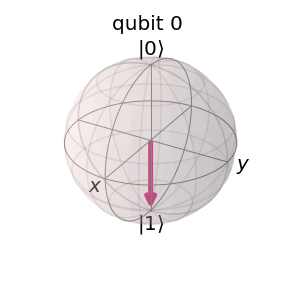
\includegraphics[scale = 0.75]{../Demonstration/img/Quantum_essentials_1.PNG}
\caption{A Bloch sphere representation of 1 qubit in the |1> state. The Bloch sphere clearly indicates that the state of a qubit has a certain probabilistic aspect to it.}
\end{figure}




superposition

entanglement

teleportation

dense coding




